\chapter{Topology optimization}
In the previous chapter, we learned how to transform a continuous elastic problem on a two-dimensional domain into a discrete problem using finite elements. 

\begin{objectives}{}{objectives_topology}
After studying this chapter and finishing the exercise, you should be able to 
\begin{itemize}[label=$\dots$]
    \item transfer solution methods from sizing problems to FEM-discretized problems
    \item solve for binary topologies using the SIMP approach
    \item discuss numerical problems in topology optimization
    \item apply filters to deal with numerical problems and manufacturing constraints
\end{itemize}
\end{objectives}

\section{Variable thickness sheet problem}
Let's consider a two-dimensional domain discretized with finite elements, in which we can adjust the thickness of each element. We may seek the best distribution of thicknesses $\mathbf{d}$ to minimize compliance $C$ with a constrained amount of material volume $V_0$. This problem can be formulated in analogy to the standard problem of sizing optimization stated in Equation \eqref{eq:size_optimization}: 

\begin{equation}
    \begin{aligned}
        \min_{\mathbf{d}} \quad & C(\mathbf{d}) = \mathbf{f} \cdot \mathbf{u}(\mathbf{d})\\
        \textrm{s.t.} \quad & \mathbf{d} \cdot \mathbf{A} - V_0 \le 0  \\
                            & \mathbf{d} \in \mathcal{D}\\
    \end{aligned}
    \label{eq:sheet_optimization}
\end{equation}

Mathematically, this problem is equivalent to the truss problem and can be solved in the same way: We formulate the Lagrangian
\begin{equation}
    \mathcal{L}(\mathbf{d}, \mu) = C(\mathbf{d}) + \mu \left( \mathbf{d} \cdot \mathbf{A} - V_0 \right) 
\end{equation}
and determine its derivative
\begin{equation}
    \frac{\partial \mathcal{L} (\mathbf{d}, \mu)}{\partial d_j} 
    = \frac{\partial C(\mathbf{d})}{\partial d_j} + \mu A_j 
\end{equation}
with 
\begin{equation}
    \frac{\partial C}{\partial d_j} = - \mathbf{u}_j(\mathbf{d})  \cdot \mathbf{k}^0_j \cdot \mathbf{u}_j(\mathbf{d}).
    \label{eq:sensitivity_sheet}
\end{equation}
In comparison to Equation \eqref{eq:compliance_sensitivity} for trusses with four degrees of freedom, the element displacement vector contains eight degrees of freedom for these 2D problems with linear quad elements ($\mathbf{u}_j \in \mathcal{R}^8, \mathbf{k}^0_j \in \mathcal{R}^{8\times 8}$). 

Just like the truss problem, the variable thickness sheet problem can be approximated using MMA with lower asymptotes only. Subsequently, it is solved with the dual method and a line search to find the Lagrange parameter $\mu$. The entire procedure is identical to Sections \ref{sec:sizing:mma} and \ref{sec:sizing:solution}, if we replace the truss cross sections $\mathbf{a}$ with element thicknesses $\mathbf{d}$ and the truss lengths $\mathbf{l}$ with element areas $\mathbf{A}$.

\begin{example}{Cantilever beam}{cantileveroptimizationexample}
    Consider a FEM cantilever beam from the previous example. Instead of just computing the displacements, we are now interested in finding the optimal thickness of each element given a volume constraint.

    We formulate the following algorithm to solve that problem: 
    \begin{enumerate}
        \item Define the cantilever FEM model with all nodes $\mathcal{N}$, elements $\mathcal{E}$, material property $E$, volume constraint $V_0$, design limits $\mathbf{d}^l, \mathbf{d}^u$ and the initial design choice $\mathbf{d}^0$.
        \item Compute the displacements $\mathbf{u}^k = \mathbf{u}(\mathbf{d}^k)$ by solving the FEM system for the current design $\mathbf{d}^k$.
        \item Compute the strain energies per area for all elements using the previously computed displacements   
        \begin{equation}
            w^k_j(\mathbf{d}^k) = \frac{1}{2}\mathbf{u}^k_j  \cdot \mathbf{k}^0_j \cdot \mathbf{u}^k_j
        \end{equation}
        \item Compute the lower asymptotes as $\mathbf{L}^k =\mathbf{d}^k - s (\mathbf{d}^u - \mathbf{d}^l)$ with $s \in (0,1)$ during the first two iterations and according to 
        \begin{equation}
            L^k_j = 
            \begin{cases}
                d^k_j - s  (d^{k-1}_j-L^{k-1}_j) & (d_j^k-d_j^{k-1})(d_j^{k-1}-d_j^{k-2}) < 0\\
                d^k_j - \frac{1}{\sqrt{s}}  (d^{k-1}_j-L^{k-1}_j) & \text{else}
            \end{cases}
        \end{equation}
        in the following iterations.
        \item Compute the lower move limit as 
        \begin{equation}
            \tilde{\mathbf{d}}^{l,k} = \max(\mathbf{d}_l,  0.9 \mathbf{L}^k + 0.1 \mathbf{d}^k)
        \end{equation}
        \item Evaluate the analytical solution
            \begin{align}
                \hat{d}_j(\mu) &= L_j^k + \sqrt{\frac{2 w_j (\mathbf{d}^k)
                (L^k_j-d^k_j)^2}{\mu A_j}} \\
                \mathbf{d}^* (\mu) &= \max\left(\tilde{\mathbf{d}}^{l,k}, \min \left(\hat{\mathbf{d}}(\mu), \mathbf{d}_u \right)\right)
            \end{align}
        \item Perform a line search to find the root $\mu^*>0$ in 
        \begin{equation}
            \frac{\partial \underline{\mathcal{L}}}{\partial \mu}(\mu) = \mathbf{A} \cdot \mathbf{d}^* (\mu) - V_0  = 0
        \end{equation}
        with Newton's method or bisection method. 
        \item Repeat with steps 2-7 until convergence or a maximum number of iterations is reached.
    \end{enumerate}

    The following image shows a result of the algorithm for the cantilever problem stated above. Black areas use the full maximum thickness $\mathbf{d}^u$ and white areas use the minimum thickness $\mathbf{d}^l$. The intermediate values are represented by different shades of gray.
    
    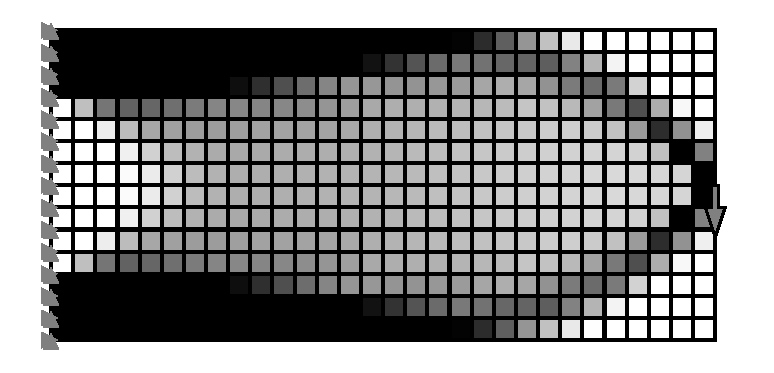
\includegraphics[width=0.9\linewidth]{figures/cantilever_fem_optimized.pdf}
       
\end{example}

\section{Solid isotropic material with penalization (SIMP)}

The problem stated in Equation \eqref{eq:sheet_optimization} is essentially a sizing optimization problem. In a topology optimization, we seek a material distribution, where each element is either completely filled or completely unfilled with material. We can formulate such a problem by reinterpreting the thickness variable as a normalized material density $\pmb{\rho}$, where $\rho_j=1$ indicates presence of material and $\rho_j=0$ indicates absence of material in element $j$. The stiffness of each element becomes a function of $\rho_j$, e.g. 
\begin{equation}
    \mathbb{C}(\rho_j)=
    \begin{cases}
        \mathbb{C} & \text{if} \quad \rho_j = 1 \\
        0          & \text{if} \quad \rho_j = 0
    \end{cases}
\end{equation}

Then, the problem statement reads
\begin{equation}
    \begin{aligned}
        \min_{\pmb{\rho}} \quad & C(\pmb{\rho}) = \mathbf{f} \cdot \mathbf{u}(\pmb{\rho})\\
        \textrm{s.t.} \quad & \pmb{\rho} \cdot \mathbf{V} - V_0 \le 0  \\
                            & \rho_j \in \{0, 1\}\\
    \end{aligned}
    \label{eq:topology_optimization}
\end{equation}

where the only change compared to Equation \eqref{eq:sheet_optimization} is the discrete nature of the design variables $\pmb{\rho}$ (and the name of the design variables). Unfortunately, the binary problem is notoriously hard to solve, because we cannot compute gradients on the solution and testing all solutions is computationally inaccessible. Hence we try to formulate a continuous relation between stiffness and normalized density that still results in a binary result. One such formulation is called \emph{Solid Isotropic Material with Penalization} (SIMP) and denoted as 
\begin{equation}
    \mathbb{C}(\rho_j)= \rho_j^p \mathbb{C}
\end{equation}
with a penalization parameter $p \ge 1$. The effect of penalization is shown in Figure \ref{fig:simp} for typical values of $p$. We may observe for $p>1$ that the stiffness per invested material is unattractive for intermediate density values. For example, choosing $\rho_j=0.5$ adds half an element volume to the total volume, but contributes only a quarter of the stiffness compared to a fully filled element. An optimization that tries to minimize compliance for a given volume will therefore rather favor elements that provide the full stiffness benefit ($\rho=1$) or do not count towards the constraint ($\rho=\rho^l$). 

\begin{figure}[!htpb]
    \centering
    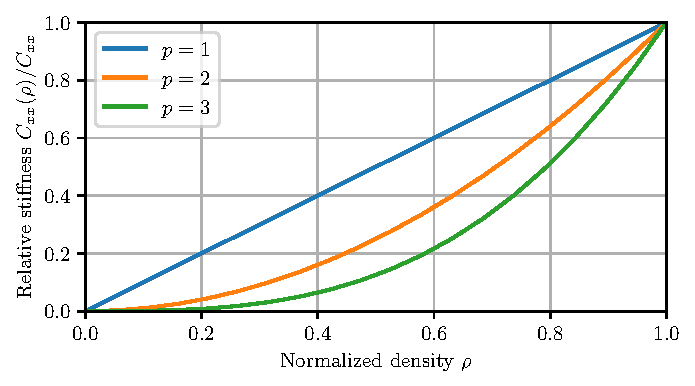
\includegraphics[width=0.7\textwidth]{figures/simp.pdf}
    \caption{Penalization factors in SIMP.}
    \label{fig:simp}
\end{figure}

Incorporating the SIMP method to the optimization is straight-forward. We just need to adjust the sensitivity (see Equation \ref{eq:sensitivity_sheet}) slightly to
\begin{equation}
    \frac{\partial C}{\partial d_j} = - p (d_j)^{p-1} \mathbf{u}_j(\mathbf{d})  \cdot \mathbf{k}^0_j \cdot \mathbf{u}_j(\mathbf{d}).
\end{equation}

\begin{example}{Cantilever beam with SIMP}{cantileversimpoptimizationexample}
    Consider a FEM cantilever beam from the previous example. We only adjust the solution in Step 6 towards 
    \begin{equation}
        \hat{d}_j(\mu) = L_j^k + \sqrt{\frac{2 w_j (\mathbf{d}^k)
        (L^k_j-d^k_j)^2}{\mu A_j}}
    \end{equation}
    and end up with the following solution:
    
    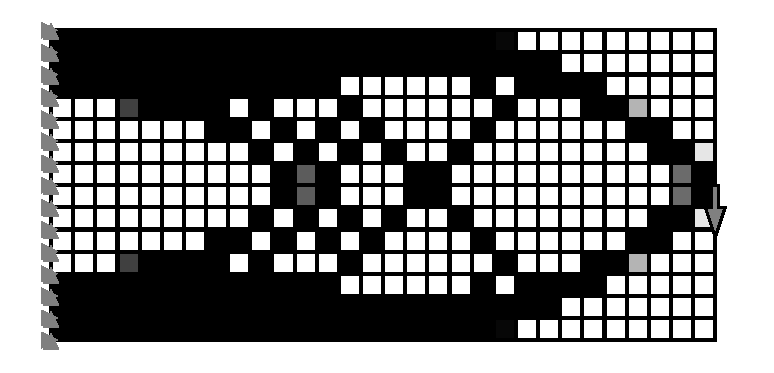
\includegraphics[width=0.9\linewidth]{figures/cantilever_fem_optimized_binary.pdf}
       
\end{example}

% discuss numerical problems and unique solution


\section{Filters}


% Filters (unique solution, no fine structures and checkerboarding)
%   - densities
%   - sensitivities (simple!)

\section{Alternative methods}

% Other methods 
%   - optimality constraints in SIMP (OC)
%   - Empirical topology optimization (SKO)
%   - Level set function 